% Chapter 3

\chapter{系统设计与实现}

本章主要介绍本系统的设计与实现,包括系统的整体架构、各个模块的功能和实现方法。

\section{系统架构概述}
本系统包含图像分析、古诗生成、古诗评价和古诗优化四个模块,基于Python语言开发,使用百度智能云提供的API接口来调用模型,整体架构如图~\ref{fig:system_architecture}所示。

\begin{figure}[h]
    \centering
    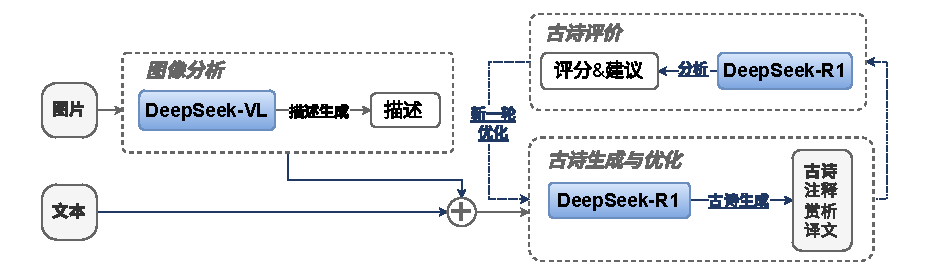
\includegraphics[width=1\textwidth]
    {figures/系统架构.pdf}\\
    \caption{系统架构}
    \label{fig:system_architecture}
  \end{figure}

\section{图像分析}

在先前的方案中,图像分析使用的是英文模型CLIP和MiniGPT-4,尽管生成的描述较精确、但无法捕捉有助于古诗创作的中国文化联想素材与情感色彩。因此,本系统使用DeepSeek-VL2\cite{wuDeepSeekVL2MixtureofExpertsVisionLanguage2024}替代之前的多模型组合方案,一步到位地为图像生成兼顾关键物体识别、整体场景信息和情感色彩的描述。(提示词见~\ref{fig:prompt_image_analysis})

在调用百度智能云的API接口时,需要提供提示词和图像的URL地址,因此还需要将用户提供的图像上传到云端,并获得可公开访问的URL。为此,使用阿里云的对象存储OSS服务,利用OSS Python SDK,将用户图像上传到云端后,生成带有过期时间的GET方法预签名URL,供后续API调用使用。

\section{古诗生成}

在先前的方案中,古诗生成使用的是ERNIE-4.0模型,其无法在遵守韵律要求的同时充分运用经典典故意象,更别说提供使用典故的注释。因此,本系统使用DeepSeek-R1\cite{deepseek-aiDeepSeekR1IncentivizingReasoning2025},提示词设计参考CRISPE框架(提示词见~\ref{fig:prompt_poem_generation})。

CRISPE框架包括六个部分:
\begin{enumerate}
  \item 能力与角色(Capacity and Role): 大模型应当具备的角色与能力。
  \item 背景信息(Insight): 为完成任务,大模型应当知晓的背景知识信息,以及用户需求的上下文语境。
  \item 指令(Statement): 大模型需要完成的任务。
  \item 输出风格(Personality): 大模型输出回复的风格、特色以及规范。
  \item 实验(Experiment): 尝试让大模型提供一些例子,以便更好地调试提示词。
\end{enumerate}

其中,最后投入使用的只包括前五个部分,而最后一个部分“实验(Experiment)”只是作调试用,方便提示词的设计迭代。

在生成古诗时,系统接收用户的文本输入\verb|user_text|,与用户输入图像的描述\verb|description|结合,同时指定古诗的体裁\verb|poem_type|(如五言绝句、七言律诗、不少于8句的排律等)。而除了古诗本身外,系统还会输出古诗的赏析、对古诗中典故的注释、以及白话文翻译,以便用户充分地理解古诗的意境、内涵和创作思路。


\section{古诗评价}

为了评价古诗的质量,本系统在自动度量方法的基础上,引入了DeepSeek-R1的评分机制。而为了使其能够给出合理、细致的评分,本文设计了一套包含五大维度的古诗评分体系(见~\ref{tab:poem_scoring}),在先前工作的基础上,这套体系强调了对子维度中分数段的详细划分,并提供对应的示例以进一步阐明评分标准。

基于这套评分体系,系统将逐一分析古诗的每个维度,给出分数和评语。此外,系统还将依照这套体系,逐一地给出修改意见,以提高古诗的质量。

\section{古诗优化}

……

在先前的工作中,古诗优化的输入只包含待改进的古诗\verb|poem|和提供的修改意见\verb|suggestion|,这会导致两个问题——其一,修改意见\verb|suggestion|中的建议往往只包含那些明显不足的方面,并不能覆盖评分体系的所有维度,因此在优化时,模型很可能会忽略那些未被提及的维度,进而导致优化后的古诗在这些方面的分数下降,顾此而失彼;其二,在古诗优化时,模型只考虑了古诗的内容和结构,却没有考虑用户的原始输入,因此优化过程也可能会偏离用户的初衷,导致生成的古诗与用户的期望相去甚远。

因此,本系统在古诗优化时,除了原古诗\verb|poem|和改进建议\verb|suggestion|外,还增加了先前对原古诗的评分\verb|evaluation|和用户的输入(文本输入\verb|user_text|与图像输入描述\verb|description|),在确保古诗优化有效性的同时,保留对用户需求的考量。

\section{项目结构}

……
<代码结构图>
……
